\chapter{Epilogue}
\label{ch:epilogue}
\renewcommand{\thefigure}{E.\arabic{figure}}

Building on experiences gained from investigations into InfextX single cell feature data such as outlined in sections \ref{sec:preliminary-res} and \ref{sub:norm-res}, \citet{Drewek2015} suggests using the random forest algorithm \citep{Breiman2001,Liaw2002} for determining which features are most influential for infection response. Random forest is chosen due to its robustness towards over-fitting and good performance under complex interactions, which both are important properties given the high dimensional, heavily correlated datasets at hand. Furthermore, an elegant estimation of variable importance is available by random forest analysis.

Predicting the results from \cgls{dtis} using all cellular features measured on the \cgls{dna} and actin channels yields an importance score assigned to each of the included features. By generating rankings per well and not aggregating data in well replicates, normalization can be reduced to mean centering. An overall importance score can be calculated in a subsequent step by averaging the respective importance scores from replicated experiments. This may alleviate some of the problems surrounding data normalization encountered in earlier analysis approaches.

\begin{knitrout}
\definecolor{shadecolor}{rgb}{0.969, 0.969, 0.969}\color{fgcolor}\begin{figure}

{\centering 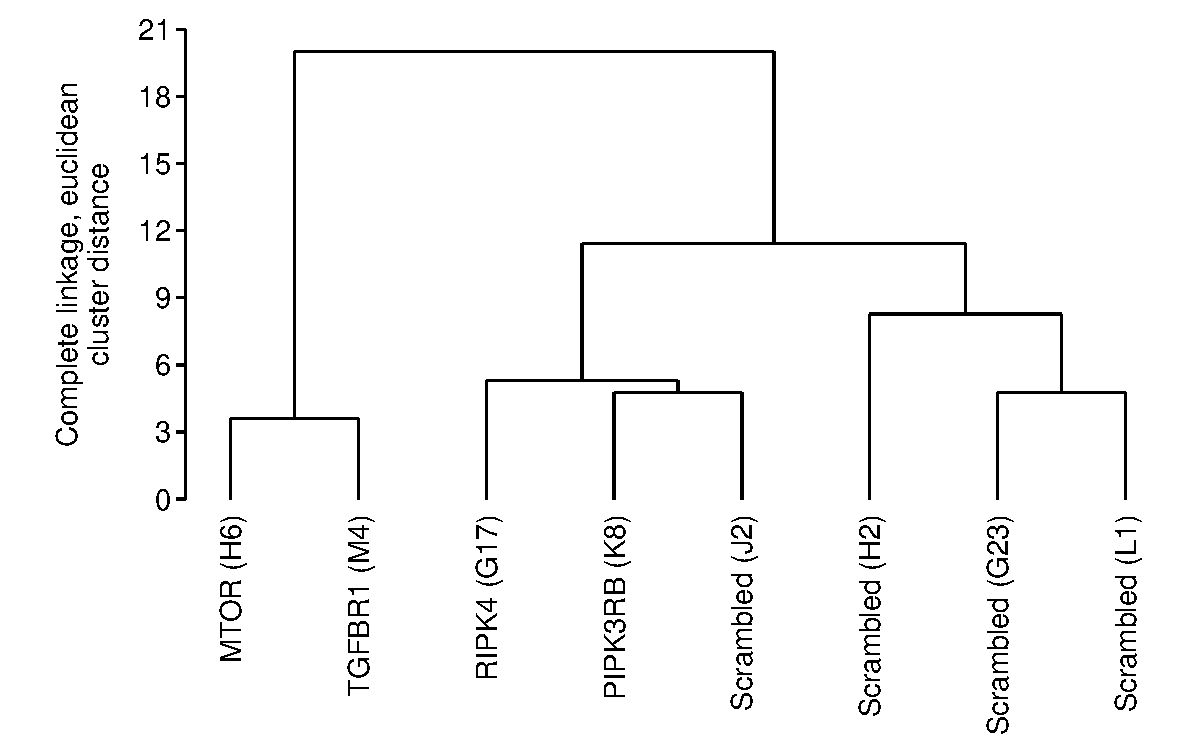
\includegraphics[width=.7\linewidth]{figures/R/forest-tree-forest-tree-1} 

}

\caption[Hierarchical clustering on averaged random forest importance scores of cellular features.]{Complete linkage hierarchical clustering performed on euclidean distances from cell feature importance scores, obtained through random forest analysis and averaged by well. For each gene and scrambled well, all available 8 replicates of the \textit{Brucella} Dharmacon unpooled dataset were considered.}\label{fig:forest-tree}
\end{figure}


\end{knitrout}



A visualization of results obtained via the described approach is shown in figure \ref{fig:forest-tree}. Similarity of overall importance scores for the \tilde 300 included cellular features is described by complete linkage hierarchical clustering based on euclidean distances. Interestingly, the two included down-hits from \cgls{pmm} analysis (see section \ref{sub:pmm}), \ACRshort{mtor} (H6) and \ACRshort{tgfbr1} (M4), are grouped closely together, as are the two selected up-hits, \ACRshort{pik3r3} (K8) and \ACRshort{ripk4} (G17). Moreover, 3 of the 4 included control wells form their own cluster (H2, G23 and L1), with the exception of scrambled well J2. Also, the well location with respect to assay plate does not seem to matter much given these results. Of course this provides only little evidence for the aptitude of random forest but may nevertheless present a promising motive to pursue this avenue further. One should certainly study a larger range of genes and it would be interesting to see to what extent known gene networks can be recovered using these methods.

\begin{knitrout}
\definecolor{shadecolor}{rgb}{0.969, 0.969, 0.969}\color{fgcolor}\begin{figure}

{\centering 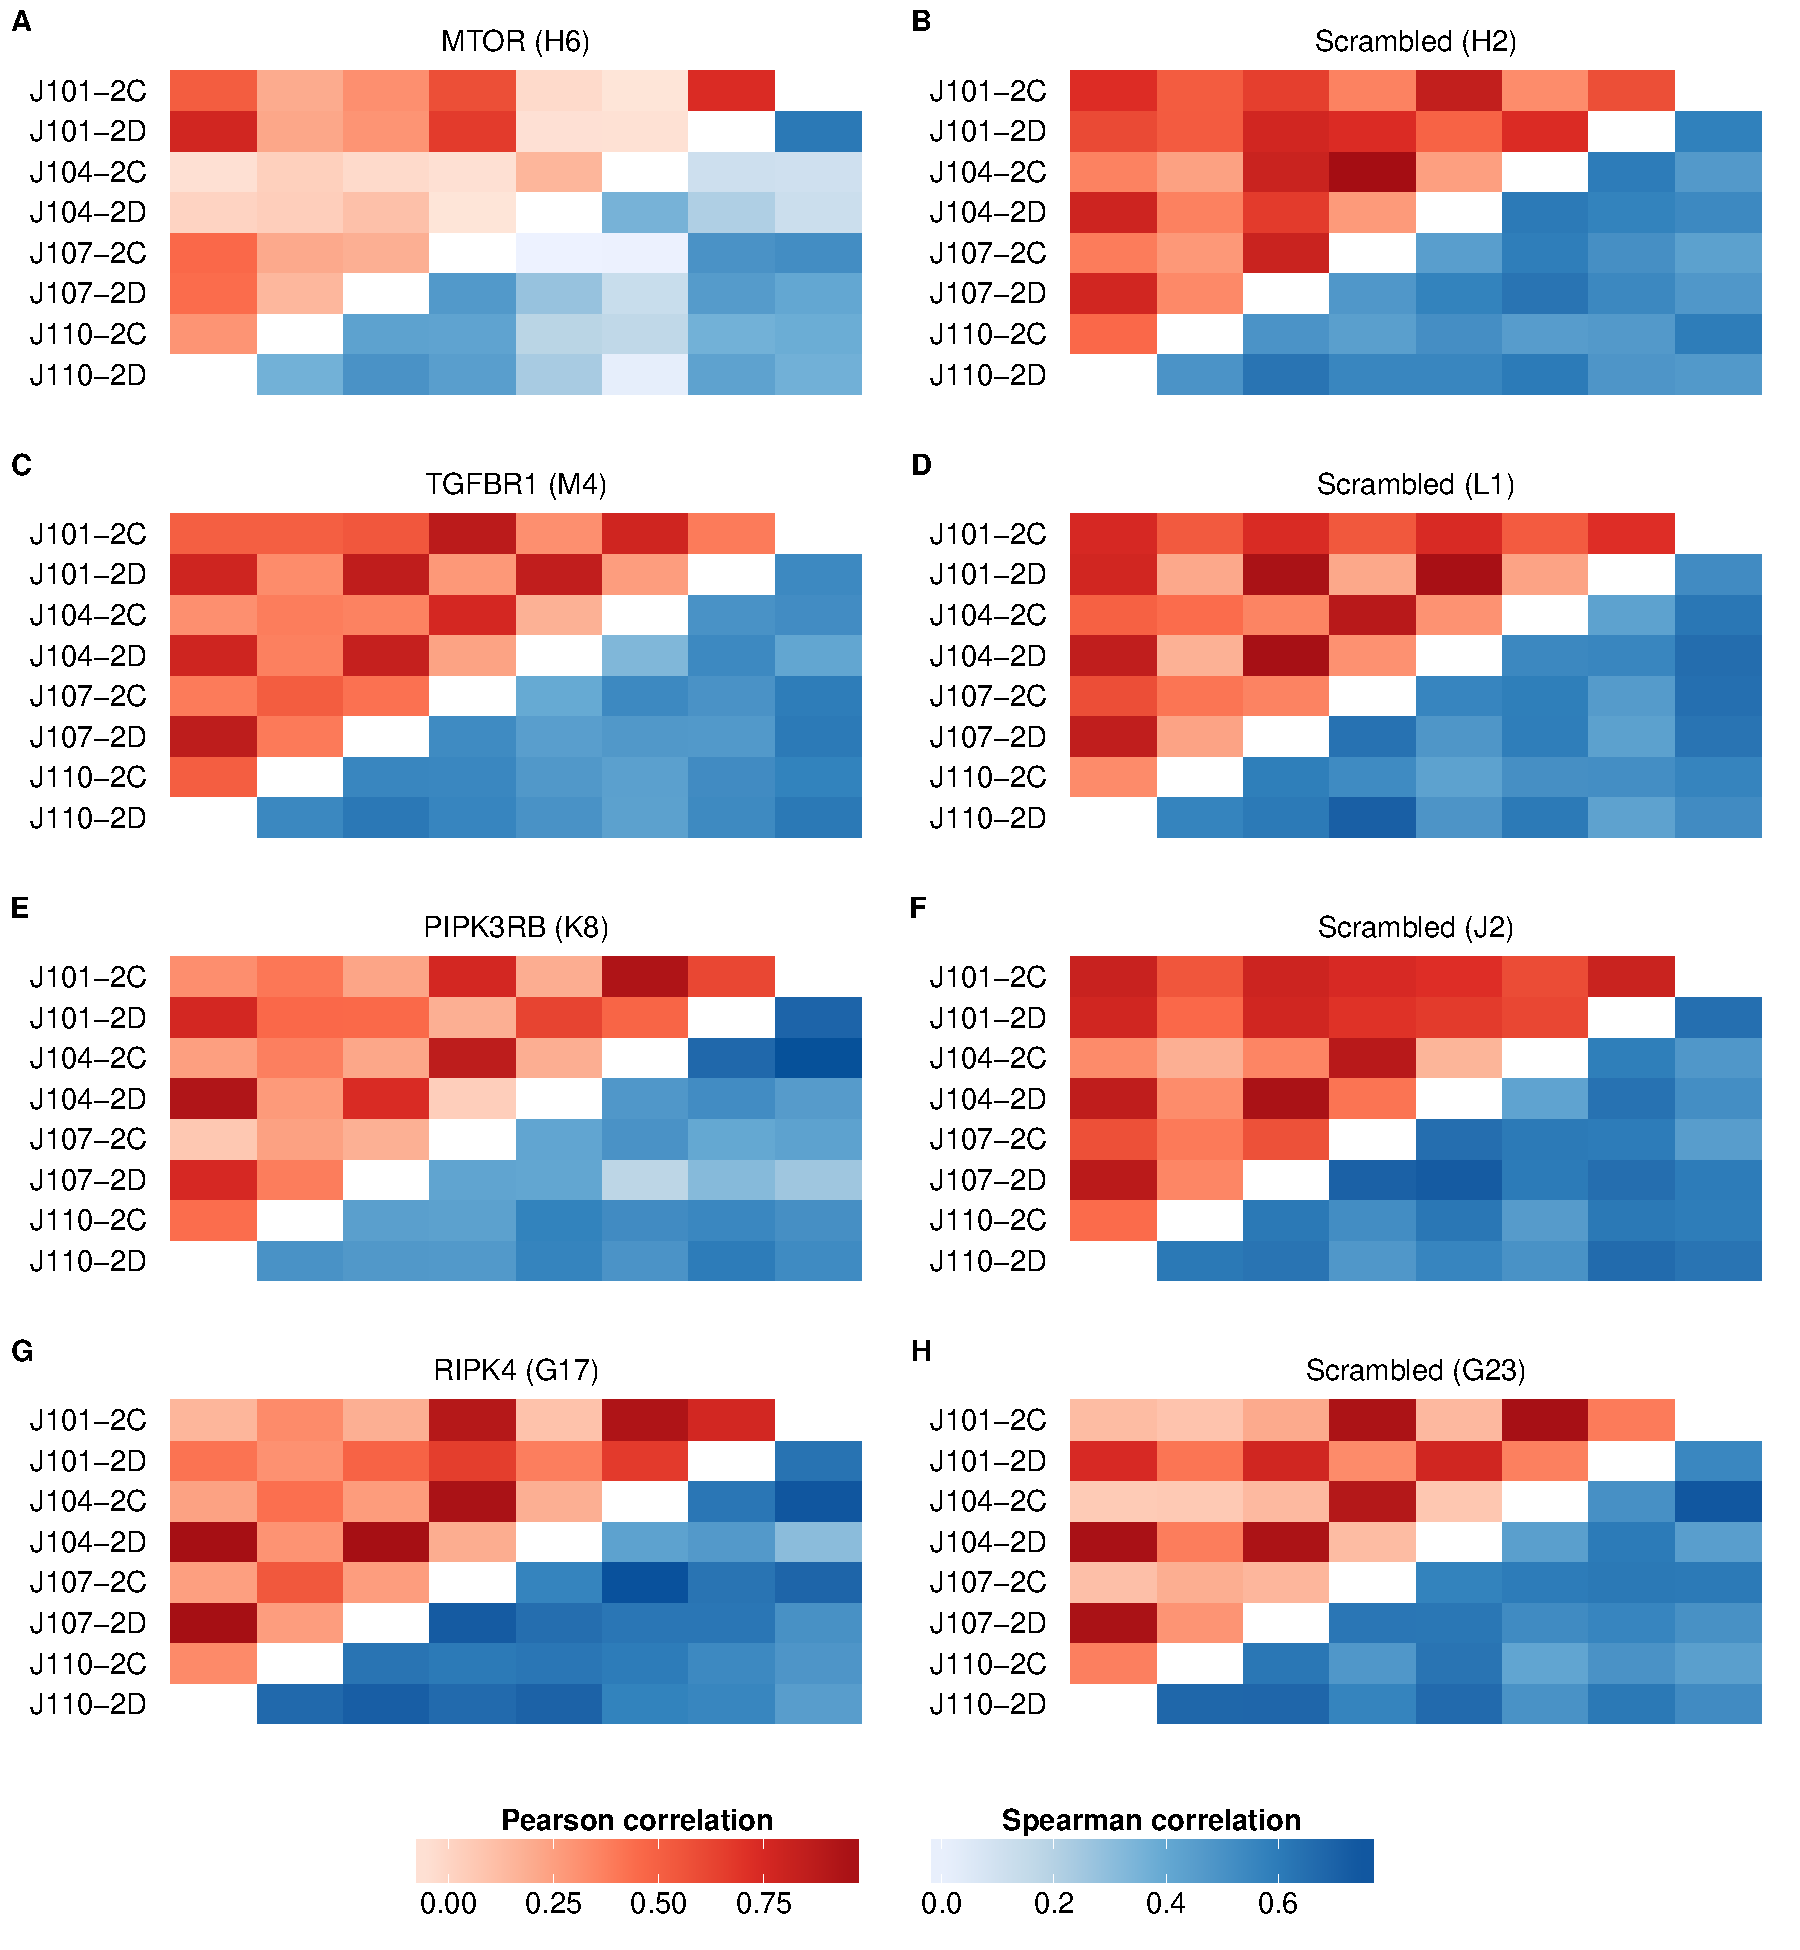
\includegraphics[width=\maxwidth]{figures/R/forest-corr-forest-corr-1} 

}

\caption[Heatmap representations of Pearson and Spearman correlation among feature importance scores obtained by random forest analysis.]{Heatmap representations of correlation matrices obtained by comparing importance scores of features as determined by random forest analysis. Red shades indicate Pearson correlation while blue shades visualize Spearman's rank correlation coefficients. For each gene and scrambled well, all available 8 replicates of the \textit{Brucella} Dharmacon unpooled dataset were considered.}\label{fig:forest-corr}
\end{figure}


\end{knitrout}



One additional possibility, which so far has not been explored and may be of value to random forest analysis, is utilizing replicates and the behavior of control wells to correct for experimental and biological noise. Looking at heatmap representations of correlation matrices (see figure \ref{fig:forest-corr}) based on importance scores (Pearson's product-moment correlation; red) and feature rankings (Spearman's rank correlation; blue) per individual well, two observations can be made: \begin{enumerate*}[label=\itshape (\arabic*)] \item there is considerable variation among replicates and \item \label{itm:scram-sim} scrambled wells behave similarly to targeted \cgls{sirna} wells, with respect to this comparison \end{enumerate*}.

Exploiting the large number of replicates available in kinome-wide screens is an opportunity not available to the analysis of genome-wide datasets which were investigated by \citeauthor{Drewek2015}. Both stability of rankings and variability of importance scores may be investigated and this could be used to remove outliers. Additionally, a more sophisticated scheme for aggregating the scores from individual wells should be developed. The current averaging can easily be improved upon, for example by giving more weight to patterns common to several wells, thus reducing the influence of deviating wells. Furthermore, aggregation of rankings within gene targets, but spanning manufacturers and possibly even pathogens could be attempted.

Observation \ref{itm:scram-sim} is mentioned because the initial presumption that the two well types somehow behave differently, perhaps with scrambled wells resulting in lower correlation coefficients due to less clear patterns, cannot be confirmed based on these results. This is not neccessarily an issue of data quality but may simply be a \cgls{sirna}-induced phenotype. It does, however, raise interesting questions: Do scrambled wells manifest some type of `background behavior' of non-specific response to \cgls{sirna} reagents? How could this source of biological noise be summarized and subtracted from targeted \cgls{sirna} wells? How do mock control wells behave and could they be exploited as well?

Already from this brief look at new developments in analysis of InfectX single cell feature data, it becomes apparent that much opportunity is present within this invaluable dataset. Further study should be able to bring to light exciting discoveries in the study of the human infectome and likely enable new ways of analyzing image-based \cgls{hts} data at single cell level.